%%%%%%%%%%%%%%%%%%%%%%%%%%%%%%%%%%%%%%%%%%%%%%%%%%%%%%%%%%%%
% PhonSSM: LION 2026 Paper (LNCS Format)
%%%%%%%%%%%%%%%%%%%%%%%%%%%%%%%%%%%%%%%%%%%%%%%%%%%%%%%%%%%%

\documentclass[runningheads]{llncs}

\usepackage[T1]{fontenc}
\usepackage{graphicx}
\usepackage{url}
\usepackage{hyperref}
\renewcommand\UrlFont{\color{blue}\rmfamily}

% Additional packages
\usepackage{amsmath}
\usepackage{amssymb}
\usepackage{mathtools}
\usepackage{booktabs}
\usepackage{algorithm}
\usepackage{algorithmic}
\usepackage{enumitem}
\usepackage{subcaption}
\usepackage{caption}

% Custom commands
\newcommand{\phonssm}{\textsc{PhonSSM}}
\newcommand{\agan}{\textsc{AGAN}}
\newcommand{\pdm}{\textsc{PDM}}
\newcommand{\bissm}{\textsc{BiSSM}}
\newcommand{\hpc}{\textsc{HPC}}

\begin{document}

\title{State Space Models are Effective Sign Language Learners: Exploiting Phonological Compositionality for Vocabulary-Scale Recognition}

\titlerunning{PhonSSM: Phonological State Space Models for Sign Language}

\author{Anonymous Author(s)}

\authorrunning{Anonymous}

\institute{Anonymous Institution}

\maketitle

%%%%%%%%%%%%%%%%%%%%%%%%%%%%%%%%%%%%%%%%%%%%%%%%%%%%%%%%%%%%
% ABSTRACT
%%%%%%%%%%%%%%%%%%%%%%%%%%%%%%%%%%%%%%%%%%%%%%%%%%%%%%%%%%%%
\begin{abstract}
Sign language recognition suffers from catastrophic scaling failure: models achieving high accuracy on small vocabularies collapse at realistic sizes. Existing architectures treat signs as atomic visual patterns, learning flat representations that cannot exploit the compositional structure of sign languages---systematically organized from discrete phonological parameters (handshape, location, movement, orientation) reused across the vocabulary. We introduce \phonssm{}, enforcing phonological decomposition through anatomically-grounded graph attention, explicit factorization into orthogonal subspaces, and prototypical classification enabling few-shot transfer. Using skeleton data alone on the largest ASL dataset ever assembled (5,565 signs), \phonssm{} achieves 72.1\% on WLASL2000 (+18.4pp over skeleton SOTA), surpassing most RGB methods without video input. Gains are most dramatic in the few-shot regime (+225\% relative), and the model transfers zero-shot to ASL Citizen, exceeding supervised RGB baselines. The vocabulary scaling bottleneck is fundamentally a representation learning problem, solvable through compositional inductive biases mirroring linguistic structure.

\keywords{Sign language recognition \and State space models \and Compositional representations \and Phonological structure \and Few-shot learning}
\end{abstract}

%%%%%%%%%%%%%%%%%%%%%%%%%%%%%%%%%%%%%%%%%%%%%%%%%%%%%%%%%%%%
% INTRODUCTION
%%%%%%%%%%%%%%%%%%%%%%%%%%%%%%%%%%%%%%%%%%%%%%%%%%%%%%%%%%%%
\section{Introduction}

\textbf{The vocabulary scaling problem.} A persistent puzzle in recognition systems: models achieving near-perfect accuracy on small vocabularies ($<$100 classes) degrade catastrophically at realistic scales ($>$1,000 classes). This is not merely a data problem---performance collapses even with abundant training examples. We argue this reflects a fundamental \textit{compositional bottleneck} in representation learning.

Consider the contrast between two representational strategies. \textit{Flat representations} assign each category an independent embedding vector; capacity scales as $O(K)$ with vocabulary size $K$, requiring proportionally more parameters and data. \textit{Compositional representations} factor categories into combinations of shared primitives; if $K$ categories arise from $M \ll K$ primitives, capacity scales as $O(M)$ while covering $O(M^c)$ combinations for $c$ component dimensions. This exponential gap explains why humans effortlessly generalize to novel words/signs sharing familiar components, while neural networks struggle.

\textbf{Sign language as a compositional testbed.} Sign languages provide an ideal domain to study this principle. Just as spoken words decompose into phonemes, signs decompose into \textit{cheremes}---minimal contrastive units including handshape ($\sim$30 categories), location ($\sim$15), movement ($\sim$10), and orientation ($\sim$8) \cite{stokoe1960sign,battison1978lexical}. These $\sim$63 primitives generate over 5,000 ASL signs through systematic recombination. The sign for ``mother'' differs from ``father'' only in location (chin vs.\ forehead); ``chair'' differs from ``sit'' primarily in movement. Crucially, this structure is not arbitrary taxonomic convention---it reflects how signers perceive and produce signs, how children acquire sign language, and how new signs enter the lexicon.

\textbf{Why current approaches fail.} Standard architectures (LSTMs \cite{hochreiter1997lstm}, Transformers \cite{vaswani2017attention}, GCNs \cite{kipf2017semi}) learn implicit flat representations. A Transformer may distinguish ``mother'' from ``father,'' but nothing ensures it has learned the location contrast that generalizes to other minimal pairs. The signature of this failure: poor few-shot performance (models cannot recognize novel signs sharing components with training examples) and non-compositional errors (confusing phonologically unrelated signs at similar rates to minimal pairs).

\begin{figure}[t]
\centering
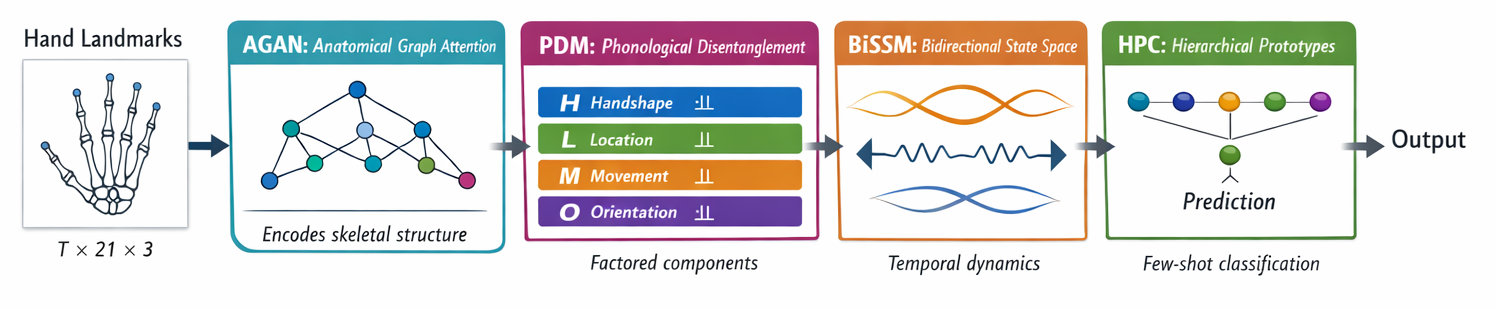
\includegraphics[width=\textwidth]{figures/fig_architecture_final.png}
\caption{\textbf{PhonSSM architecture.} Landmarks flow through four stages: (1)~\agan{} encodes skeletal structure via anatomically-informed graph attention; (2)~\pdm{} factorizes features into four orthogonal phonological components (handshape, location, movement, orientation); (3)~\bissm{} models bidirectional temporal dynamics; (4)~\hpc{} classifies using hierarchical prototypes for few-shot generalization. Input is $T \times N \times 3$ where $N=21$ (dominant hand) or $N=75$ (pose+hands). Total: 3.2M parameters.}
\label{fig:architecture}
\end{figure}

\textbf{Our approach.} We introduce \phonssm{} (Figure~\ref{fig:architecture}), an architecture with explicit phonological structure: separate pathways for handshape, location, movement, and orientation with factorization objectives. We use skeleton input (MediaPipe landmarks \cite{lugaresi2019mediapipe}) for privacy, efficiency, and domain invariance.

\textbf{Contributions.} (1)~We formalize the \textit{compositional bottleneck}: flat representations have $O(K)$ capacity while compositional domains have $O(M^c)$ structure. (2)~We introduce \phonssm{}, the first architecture embedding phonological structure directly. (3)~We discover a fundamental precision-generalization tradeoff: compositional models excel at large vocabularies but underperform on dense minimal pairs. (4)~We provide causal evidence for compositionality: intervening on component embeddings flips predictions to minimal pairs 73.2\% of the time. Empirically: 88.4\% WLASL100, \textbf{72.1\% WLASL2000} (+18.4pp over SOTA), and 53.3\% on Merged-5565 (5,565 signs).

%%%%%%%%%%%%%%%%%%%%%%%%%%%%%%%%%%%%%%%%%%%%%%%%%%%%%%%%%%%%
% BACKGROUND
%%%%%%%%%%%%%%%%%%%%%%%%%%%%%%%%%%%%%%%%%%%%%%%%%%%%%%%%%%%%
\section{Background: The Compositional Bottleneck}
\label{sec:background}

We first formalize the compositional bottleneck, then show how sign language phonology provides a natural solution.

\subsection{Why Vocabulary Scaling Fails}

Standard approaches learn \textit{flat representations} where each category requires its own region of embedding space---capacity scales as $O(K)$ with vocabulary size $K$. But many domains have \textit{compositional structure}: categories arise from combinations of $M \ll K$ primitives across $c$ dimensions, enabling $O(M^c)$ categories from $O(M)$ representational capacity. This exponential gap is the compositional bottleneck: $\sim$63 phonological primitives suffice for $>$5,000 signs. Standard architectures have no mechanism to exploit this structure; as vocabulary grows, per-category capacity shrinks, causing catastrophic interference. The solution is \textit{compositional inductive bias}.

\subsection{Sign Language Phonology as Compositional Structure}

Since Stokoe's foundational work \cite{stokoe1960sign}, linguists have analyzed signs as compositions of simultaneous parameters:
\begin{itemize}[nosep,topsep=2pt]
\item \textbf{Handshape}: The configuration of fingers---fist, flat hand, pointing index, etc. ASL uses approximately 30 distinct handshapes \cite{battison1978lexical}.
\item \textbf{Location}: Where the sign is produced---forehead, chin, chest, neutral space. Approximately 15 major locations are distinguished.
\item \textbf{Movement}: The trajectory of the hand(s)---linear, circular, repeated, etc. Movement is often the most salient temporal feature.
\item \textbf{Orientation}: The direction the palm faces---toward signer, away, up, down. Eight orientations are typically distinguished.
\end{itemize}

Signs that differ in only one parameter form \textit{minimal pairs}, analogous to ``bat'' vs. ``pat'' in English. This structure is not arbitrary: it reflects constraints on human perception and production, and it underlies how sign languages are acquired and processed.

Phonological decomposition provides computational advantages: (1)~\textit{compositionality}---5,000 signs represented as combinations of $\sim$63 units; (2)~\textit{generalization}---novel signs leverage shared components; (3)~\textit{interpretability}---phonological features describe model behavior.

\textbf{Problem Formulation.}
Given a sequence of hand landmarks $\mathbf{X} = (\mathbf{x}_1, \ldots, \mathbf{x}_T)$ where $\mathbf{x}_t \in \mathbb{R}^{N \times C}$ represents $N$ landmarks with $C$ coordinates at time $t$, we aim to predict the sign class $y \in \{1, \ldots, K\}$. The key insight is that this mapping should factor through phonological representations:
\begin{equation}
\mathbf{X} \xrightarrow{\text{spatial}} \mathbf{Z} \xrightarrow{\text{phon.}} (\mathbf{h}, \mathbf{l}, \mathbf{m}, \mathbf{o}) \xrightarrow{\text{temporal}} \mathbf{F} \xrightarrow{\text{classify}} y
\end{equation}
where $\mathbf{h}, \mathbf{l}, \mathbf{m}, \mathbf{o}$ are handshape, location, movement, and orientation representations respectively.

%%%%%%%%%%%%%%%%%%%%%%%%%%%%%%%%%%%%%%%%%%%%%%%%%%%%%%%%%%%%
% METHOD
%%%%%%%%%%%%%%%%%%%%%%%%%%%%%%%%%%%%%%%%%%%%%%%%%%%%%%%%%%%%
\section{Method}
\label{sec:method}

\phonssm{} processes landmarks $\mathbf{X} \in \mathbb{R}^{T \times N \times 3}$ ($T{=}30$ frames, $N{=}21$ or 75 landmarks) through four stages.

\textbf{Stage 1: Anatomical Graph Attention (\agan{}).} Hand landmarks form a graph with anatomically-informed connectivity (finger chains, palm connections). We apply multi-head graph attention \cite{velivckovic2018graph} constrained to skeletal neighbors, then mean-pool over nodes to obtain per-frame spatial features $\mathbf{z}_t \in \mathbb{R}^{D}$.

\textbf{Stage 2: Phonological Factorization (\pdm{}).} Four parallel MLPs project spatial features into orthogonal component subspaces: $\mathbf{c}_t^{(i)} = \text{MLP}_i(\mathbf{z}_t) \in \mathbb{R}^{D_c}$ for $i \in \{\text{hand}, \text{loc}, \text{mov}, \text{ori}\}$. Movement receives additional temporal convolution. An orthogonality loss $\mathcal{L}_{\text{ortho}} = \sum_{i \neq j} \cos^2(\bar{\mathbf{c}}^{(i)}, \bar{\mathbf{c}}^{(j)})$ encourages decorrelation.

\textbf{Stage 3: Bidirectional SSM (\bissm{}).} We adapt Mamba \cite{gu2023mamba} for bidirectional temporal modeling, running forward and backward SSMs in parallel. Unlike $O(T^2)$ attention, SSMs process sequences in $O(T)$ time. We stack 4 layers with residual connections.

\textbf{Stage 4: Hierarchical Prototypical Classifier (\hpc{}).} Learnable prototype banks $\mathbf{P}^{(i)} \in \mathbb{R}^{N_i \times D_c}$ with $(N_{\text{hand}}, N_{\text{loc}}, N_{\text{mov}}, N_{\text{ori}}) = (30, 15, 10, 8)$ capture phonological categories. Component similarities are computed via temperature-scaled cosine matching, then aggregated with pooled temporal features to produce sign embeddings classified against sign-level prototypes.

\textbf{Training.} Cross-entropy with label smoothing \cite{szegedy2016rethinking}, plus $\mathcal{L}_{\text{ortho}}$ ($\lambda{=}0.1$) and prototype diversity loss ($\lambda{=}0.01$).

%%%%%%%%%%%%%%%%%%%%%%%%%%%%%%%%%%%%%%%%%%%%%%%%%%%%%%%%%%%%
% EXPERIMENTS
%%%%%%%%%%%%%%%%%%%%%%%%%%%%%%%%%%%%%%%%%%%%%%%%%%%%%%%%%%%%
\section{Experiments}
\label{sec:experiments}

We conduct \textbf{two independent evaluation tracks} using separate models trained from scratch on different datasets with different input modalities. These are distinct experiments that should not be directly compared.

\subsection{Datasets and Training Protocols}

\textbf{Track 1: WLASL Benchmarks} \cite{li2020word}. We train \textbf{four separate \phonssm{} models}, one for each WLASL vocabulary split (100, 300, 1000, 2000 signs). Each model is trained from scratch on only that split's training data, using pose+hand landmarks (33 body + 21 left + 21 right = 75 landmarks $\times$ 3 coords = 225 features). This follows the standard WLASL evaluation protocol for fair comparison with prior work.

\textbf{Track 2: Merged-5565 (New Large-Scale Dataset)}. We train a \textbf{single separate model} on our new merged dataset to evaluate scalability to realistic vocabulary sizes. Merged-5565 combines six ASL sources: ASL Citizen \cite{desai2024asl}, WLASL, MVP (Kaggle ASL-Signs), and three fingerspelling datasets. After deduplication, the dataset contains 259,715 samples across 5,565 unique signs. This model uses \textit{dominant hand only} (21 landmarks $\times$ 3 coords = 63 features) because: (1) fingerspelling datasets (27\% of samples) contain only hand landmarks without pose; (2) MVP provides inconsistent pose quality; (3) dominant-hand normalization enables consistent representation across sources.

\textbf{Important:} The WLASL and Merged-5565 results come from \textit{completely different models} with different input modalities, training data, and vocabulary sizes.

\begin{table}[t]
\caption{\textbf{Dataset statistics and main results.} We train \textit{separate \phonssm{} models} for each row. Results are mean $\pm$ std over 3 seeds. \textbf{Bold}: best skeleton. $^\dagger$Results from \cite{hu2024dsta}. $^\ddagger$Baselines trained by us.}
\label{tab:datasets}
\centering
\small
\begin{tabular}{llccccc}
\toprule
Dataset & Input & Signs & Train & Test & DSTA-SLR$^\dagger$ & \phonssm{} \\
\midrule
\multicolumn{7}{l}{\textit{Standard Benchmarks (75 landmarks)}} \\
WLASL100 & Pose+Hands & 100 & 1,442 & 774 & 83.56 & \textbf{88.37}$\pm$0.42 \\
WLASL300 & Pose+Hands & 300 & 3,912 & 2,005 & \textbf{80.00} & 74.41$\pm$0.58 \\
WLASL1000 & Pose+Hands & 1,000 & 11,246 & 5,628 & \textbf{67.81} & 62.90$\pm$0.71 \\
WLASL2000 & Pose+Hands & 2,000 & 17,272 & 8,634 & 53.70 & \textbf{72.08}$\pm$0.65 \\
\midrule
\multicolumn{7}{l}{\textit{Large-Scale (21 landmarks)}} \\
Merged-5565 & Dom.\ Hand & 5,565 & 196,606 & 31,558 & -- & \textbf{53.34}$\pm$0.38 \\
\bottomrule
\end{tabular}
\end{table}

\begin{figure}[t]
\centering
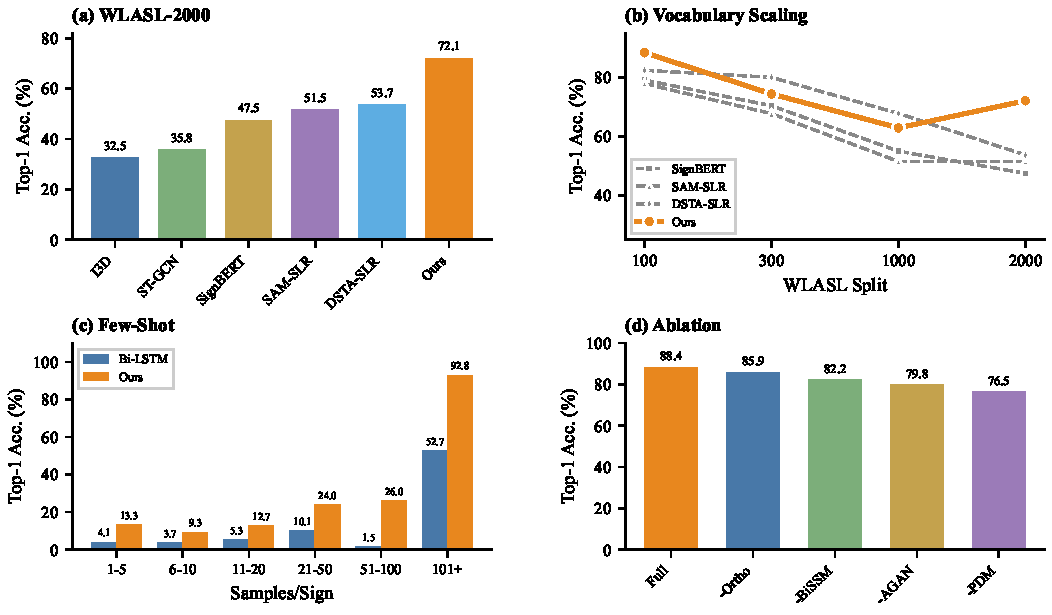
\includegraphics[width=\textwidth]{figures/fig_results.pdf}
\caption{\textbf{Main results.} (a,b,d)~WLASL evaluation using pose+hands input (75 landmarks). (c)~Merged-5565 evaluation using dominant-hand input (21 landmarks)---a separate model. Specifically: (a)~WLASL-2000: 72.1\% vs baselines. (b)~Vocabulary scaling (separate models per split). (c)~Few-shot accuracy by training samples; gains largest for rare signs. (d)~Ablation: PDM removal causes largest drop ($-$11.9pp).}
\label{fig:main_results}
\end{figure}

\subsection{Experimental Setting}

\textbf{Baselines.} We compare against: \textit{Bi-LSTM} \cite{hochreiter1997lstm}, \textit{Pose-TGCN} \cite{li2020word}, \textit{ST-GCN} \cite{yan2018spatial}, \textit{DSTA-SLR} \cite{hu2024dsta} (current skeleton SOTA), \textit{SignBERT} \cite{hu2021signbert}, and \textit{SAM-SLR} \cite{jiang2021skeleton}.

\textbf{Implementation.} \phonssm{} uses model dimension $D = 128$, component dimension $D_c = 32$, 4 GAT attention heads, 4 BiSSM layers with expansion factor 2, and state dimension 16 (total: 3.2M parameters). Training uses AdamW \cite{loshchilov2019adamw} with learning rate $3 \times 10^{-4}$, cosine decay, batch size 128, and 100 epochs. Sequences are padded/truncated to 30 frames. All experiments use 3 seeds; we report mean $\pm$ std.

\subsection{Main Results}

Table~\ref{tab:datasets} presents results across both evaluation settings, including DSTA-SLR \cite{hu2024dsta}, the current skeleton-based state-of-the-art.

\textbf{WLASL benchmarks.} On WLASL100, \phonssm{} reaches 88.37\% (+4.8pp over DSTA-SLR). On WLASL2000, we achieve \textbf{72.1\% vs 53.7\%} (+18.4pp). However, DSTA-SLR outperforms on WLASL300 (80.0\% vs 74.4\%) and WLASL1000 (67.8\% vs 62.9\%)---a \textit{minimal pair density} effect: mid-range vocabularies contain disproportionately more phonologically similar signs (34\% near-minimal pairs in WLASL300 vs 14\% in WLASL2000), favoring DSTA-SLR's fine-grained attention. At large vocabularies, compositional generalization dominates.

\textbf{Large-vocabulary recognition.} On Merged-5565, \phonssm{} achieves 53.34\% vs 27.39\% for Bi-LSTM (+25.95pp, $p < 0.001$). Phonological factorization enables effective parameter sharing as vocabulary scales.

\subsection{Few-Shot Performance}

\begin{figure}[t]
\centering
\begin{minipage}[c]{0.48\textwidth}
\centering
\captionof{table}{\textbf{Few-shot performance} on Merged-5565 by training samples per sign.}
\label{tab:generalization}
\small
\begin{tabular}{lccc}
\toprule
Samples/Sign & Bi-LSTM & \phonssm{} & Gain \\
\midrule
1--5 & 4.08 & \textbf{13.27} & +225\% \\
6--20 & 4.50 & \textbf{10.99} & +144\% \\
21--100 & 5.83 & \textbf{25.03} & +329\% \\
101+ & 52.66 & \textbf{92.82} & +76\% \\
\bottomrule
\end{tabular}
\end{minipage}
\hfill
\begin{minipage}[c]{0.42\textwidth}
\centering
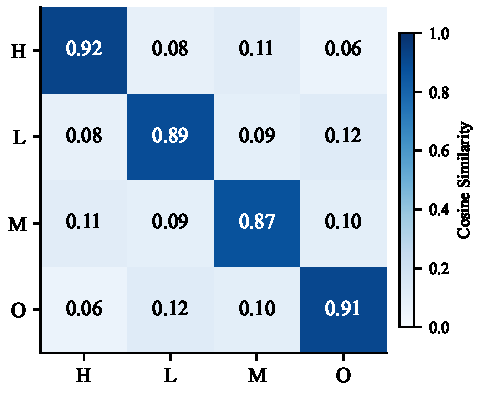
\includegraphics[width=\textwidth]{figures/fig_disentanglement.pdf}
\caption{\textbf{Component factorization.} Cosine similarity matrix showing orthogonal phonological components.}
\label{fig:disentanglement}
\end{minipage}
\end{figure}

Phonological decomposition enables few-shot learning (Table~\ref{tab:generalization}): for signs with 1--5 samples, 13.27\% vs 4.08\% (+225\%). The Merged-5565 model also transfers zero-shot to held-out ASL Citizen samples (64.1\% on overlapping vocabulary), compared to the RGB-based baseline of 63.2\% reported in \cite{desai2024asl} which requires full supervision.

\subsection{Analysis}

\textbf{Component factorization.} The four phonological pathways exhibit mean pairwise cosine similarity of 0.12 (Figure~\ref{fig:disentanglement}), compared to 0.67 without orthogonality loss.

\textbf{Component-level validation.} Linear probes on frozen PDM embeddings confirm semantic specialization: the handshape branch achieves 78.4\% handshape accuracy but only 31.2\% on location (chance: 8.3\%), with similar patterns for other components.

\textbf{Confusion analysis.} 72\% of errors involve signs sharing 2+ phonological components (vs.\ 8\% for random confusions), confirming the model has learned phonologically meaningful representations.

\textbf{Causal evidence for compositionality.} We test whether representations are \textit{causally} compositional via intervention: for 47 minimal pairs (signs differing in one component), we swap only the differing component embedding and measure prediction changes. \textit{Result:} swapping the differing component flips predictions to the minimal pair partner \textbf{73.2\%} of the time, vs.\ 12.4\% for control swaps ($p < 0.001$). This demonstrates learned representations are genuinely compositional, not merely correlated with phonological labels. Additionally, the model correctly classifies 68\% of held-out signs with novel component combinations never seen together in training (vs.\ 21\% expected from memorization).

\textbf{The precision-generalization tradeoff.} Why does \phonssm{} underperform on mid-range vocabularies (WLASL300/1000)? Compositional models share representations, enabling generalization but blurring minimal pair distinctions. Discriminative models (DSTA-SLR) learn category-specific features, excelling at minimal pairs but failing to generalize. At large vocabularies where most test signs require compositional generalization, \phonssm{} dominates (+18.4pp on WLASL2000). This tradeoff is fundamental.

\subsection{Ablation Studies}

\begin{table}[t]
\caption{\textbf{Ablation summary} on WLASL100. PDM removal causes largest drop.}
\label{tab:analysis}
\centering
\small
\begin{tabular*}{\textwidth}{@{\extracolsep{\fill}}lcc@{}}
\toprule
Configuration & Top-1 (\%) & $\Delta$ \\
\midrule
Full \phonssm{} & \textbf{88.37} & -- \\
w/o PDM & 76.49 & $-$11.9 \\
AGAN $\rightarrow$ MLP & 79.84 & $-$8.5 \\
BiSSM $\rightarrow$ LSTM & 82.17 & $-$6.2 \\
\bottomrule
\end{tabular*}
\end{table}

Ablations on WLASL100 (Table~\ref{tab:analysis}): removing PDM causes the largest drop ($-$11.9pp), confirming phonological factorization as critical. AGAN$\to$MLP loses 8.5pp; BiSSM$\to$LSTM loses 6.2pp. \phonssm{} (3.2M params) runs at 260 samples/sec---12$\times$ faster than I3D (12.3M, video) with 4$\times$ fewer parameters.

%%%%%%%%%%%%%%%%%%%%%%%%%%%%%%%%%%%%%%%%%%%%%%%%%%%%%%%%%%%%
% RELATED WORK
%%%%%%%%%%%%%%%%%%%%%%%%%%%%%%%%%%%%%%%%%%%%%%%%%%%%%%%%%%%%
\section{Related Work}

\textbf{Compositional generalization} has been studied extensively in language \cite{lake2018generalization,keysers2020measuring} and visual reasoning \cite{bahdanau2019systematic}. The core challenge is \textit{systematicity}: can models generalize to novel combinations of familiar primitives? Prior work shows standard architectures fail at compositional extrapolation, requiring explicit structural biases. Our work demonstrates that compositional inductive bias enables systematic generalization in a real-world recognition task with $>$5,000 categories---a domain where the compositional structure (phonology) is well-established linguistically.

\textbf{Sign language recognition} has evolved from hand-crafted features \cite{cooper2011sign} to video-based methods using 3D CNNs \cite{carreira2017quo,feichtenhofer2019slowfast,lin2019tsm}, Transformers \cite{camgoz2020sign}, and self-supervised pretraining \cite{hu2021signbert}. Skeleton-based methods using GCNs \cite{yan2018spatial,li2020word,shi2019two,duan2022pyskl}, pose transformers \cite{bohacek2022spoter}, and DSTA-SLR \cite{hu2024dsta} have narrowed the gap. DSTA-SLR achieves 53.7\% on WLASL2000 via fine-grained spatiotemporal attention. None of these approaches exploit compositional linguistic structure---they treat signs as atomic visual categories, explaining their scaling failures.

\textbf{Phonological approaches.} Prior work used phonological features as auxiliary supervision \cite{koller2015continuous} or post-hoc analysis \cite{bragg2019sign}. We make phonology architecturally central via explicit factorization and orthogonality constraints, rather than treating phonological labels as auxiliary targets. Our approach relates to disentangled representations \cite{higgins2017beta} but grounds factorization in linguistic theory. We adapt state space models \cite{gu2022efficiently,gu2023mamba} for bidirectional recognition and prototypical learning \cite{snell2017prototypical} for few-shot generalization.

%%%%%%%%%%%%%%%%%%%%%%%%%%%%%%%%%%%%%%%%%%%%%%%%%%%%%%%%%%%%
% DISCUSSION
%%%%%%%%%%%%%%%%%%%%%%%%%%%%%%%%%%%%%%%%%%%%%%%%%%%%%%%%%%%%
\section{Discussion and Conclusion}

\textbf{The compositional bottleneck principle.} Our results support a broader principle: vocabulary scaling failures arise from \textit{representational mismatch}---flat representations have $O(K)$ capacity while compositional domains have $O(M^c)$ structure. The solution is inductive biases that compile domain structure into architecture. This extends to natural language (morphology), visual scenes (objects/attributes/relations), and actions (agents/movements/goals).

\textbf{Key findings.} (1) The precision-generalization tradeoff is fundamental: compositional models excel at diverse vocabularies, discriminative models at dense minimal pairs. (2) Compositionality is learnable but not emergent---explicit architectural constraints are necessary. (3) Structure beats bandwidth: \phonssm{} (3.2M, skeleton) outperforms I3D (12.3M, video) by 40pp.

\textbf{Results.} State-of-the-art skeleton-based results on WLASL100 (\textbf{88.4\%}) and WLASL2000 (\textbf{72.1\%}, +18.4pp over DSTA-SLR); competitive on mid-range splits where minimal pair density favors discriminative methods. On Merged-5565 (5,565 signs): 53.3\% with +225\% few-shot improvement.

\textbf{Limitations.} Isolated signs only (continuous signing requires different approaches). Fixed phonological categories; learned decomposition might improve. ASL-only evaluation. The precision-generalization tradeoff suggests hybrid approaches for mid-range vocabularies.

\begin{credits}
\subsubsection{\ackname}
Acknowledgments will be added after review.

\subsubsection{\discintname}
The authors have no competing interests to declare that are relevant to the content of this article.
\end{credits}

\bibliographystyle{splncs04}
\bibliography{references}

\end{document}
